% ChinaVis 2026 · 赛题 1-I 答题卡（带图交付件） · xelatex 编译
\documentclass[11pt]{article}
\usepackage[a4paper,margin=2.2cm]{geometry}
\usepackage{fontspec}
\usepackage{xeCJK}
\setCJKmainfont{Noto Serif CJK SC}
\setCJKsansfont{Noto Sans CJK SC}
\usepackage{amsmath}
\usepackage{graphicx}
\graphicspath{{figures/}}
\usepackage{titlesec}
\usepackage{xcolor}
\definecolor{vermilion}{HTML}{C0392B}
\usepackage[colorlinks=true,linkcolor=vermilion,urlcolor=vermilion]{hyperref}
\usepackage{caption}
\captionsetup{font=small,labelfont={bf,color=vermilion}}
\titleformat{\section}{\Large\bfseries\color{vermilion}}{\thesection}{0.6em}{}
\titlespacing{\section}{0pt}{1.1em}{0.5em}
\setlength{\parskip}{0.35em}
\setlength{\parindent}{0pt}
\renewcommand{\baselinestretch}{1.12}

\title{\textbf{ChinaVis Data Challenge 2026 $\cdot$ 赛题 1-I「戏韵万象」答题卡}}
\author{戏韵 $\cdot$ 梨园谱系 —— 京剧剧本可视分析系统}
\date{数据可视化 2026 课程考核作品}

\begin{document}
\maketitle

\noindent\textbf{使用工具：}Python(FastAPI)、React + Vite、ECharts/D3、jieba、scikit-learn、networkx、PyMuPDF；
自研软件「戏韵 $\cdot$ 梨园谱系——京剧剧本可视分析系统」（开篇导览 + 总览 + 任务一$\sim$五 + 双剧对比 + 结语余韵，共九个联动模块）。
\textbf{数据：}竞赛 1-I 京剧数据集全部 38 个来源集合、1473 部剧本 PDF（100\% 解析），7656 个标注角色、360{,}223 条对白，全部使用。

\vspace{0.4em}\hrule\vspace{0.6em}

\section{角色行当分类与时期演化}
\textbf{方法与可信度：}从「主要角色」块解析出 \textbf{7656} 个行当标注，其中 \textbf{7428} 个与对白说话人精确匹配，作为训练实例；末并入生，杂作为群演辅助类。特征包括唱/念/白占比、台词量、出场场次、共现度、性别/年龄身份关键词和台词 TF-IDF。用逻辑回归 Pipeline 训练，实例级 5 折 \textbf{macro-F1=0.704}（旦0.85、生0.79、丑0.69、净0.68），按剧目分组验证 \textbf{0.696}，据此推断 \textbf{15034} 个未标注出场角色。推断置信度高/中/低分别为 \textbf{5670/4129/5235}，低置信样本在系统中标为「待核」，不作为强证据。为说明分数是否够用，给出基线对照（多数类 0.118、随机森林 0.552）与概率校准（多类 Brier=0.349 与可靠性曲线）。

\textbf{特征↔行当模式：}旦行唱占比最高（0.045）且女性/亲属称谓显著；丑行几乎全为白（0.90），口语化插科打诨词更多；净行多「孤家/俺/哇呀呀」等威猛粗豪表达；生行多「寡人/贤弟/孩儿」等君臣、父子、兄弟称谓。生旦共现度和台词量较高，杂类台词少、群演名命中高。表演程式、身份性别与台词风格共同构成可解释分类依据。

\textbf{时期演化：}以来源集合/出处年份作为时期代理（清末民国/建国初期/当代，标注实例 n=3693/3378/357）。净行占比持续下降（0.224→0.212→0.163），丑行当代上升（0.166→0.136→0.207），杂行当代也增多（0.001→0.036）。卡方检验显示时期与行当关联统计显著（$\chi^2$=39.2, $p$=6.5e-7），但 Cramér's V=0.052 表明效应极弱——诚实结论是行当结构总体稳定。细分行当推断仅对生（5 折 macro-F1 0.733）/旦（0.560）建模，净/丑标注稀疏故仅展示。

\textbf{误判结构分析（混淆矩阵，零重训）：}将交叉验证混淆矩阵按行归一为召回视角，最大误判集中在\textbf{生↔净}（生→净 411 例、净→生 374 例；二者同以念白为主、舞台气质相近），杂行样本稀少召回最低——误判结构与表演型重叠一致，说明 macro-F1 上限源自数据本身的行当边界模糊而非模型缺陷，并为人工复核给出优先级。

\begin{figure}[h]\centering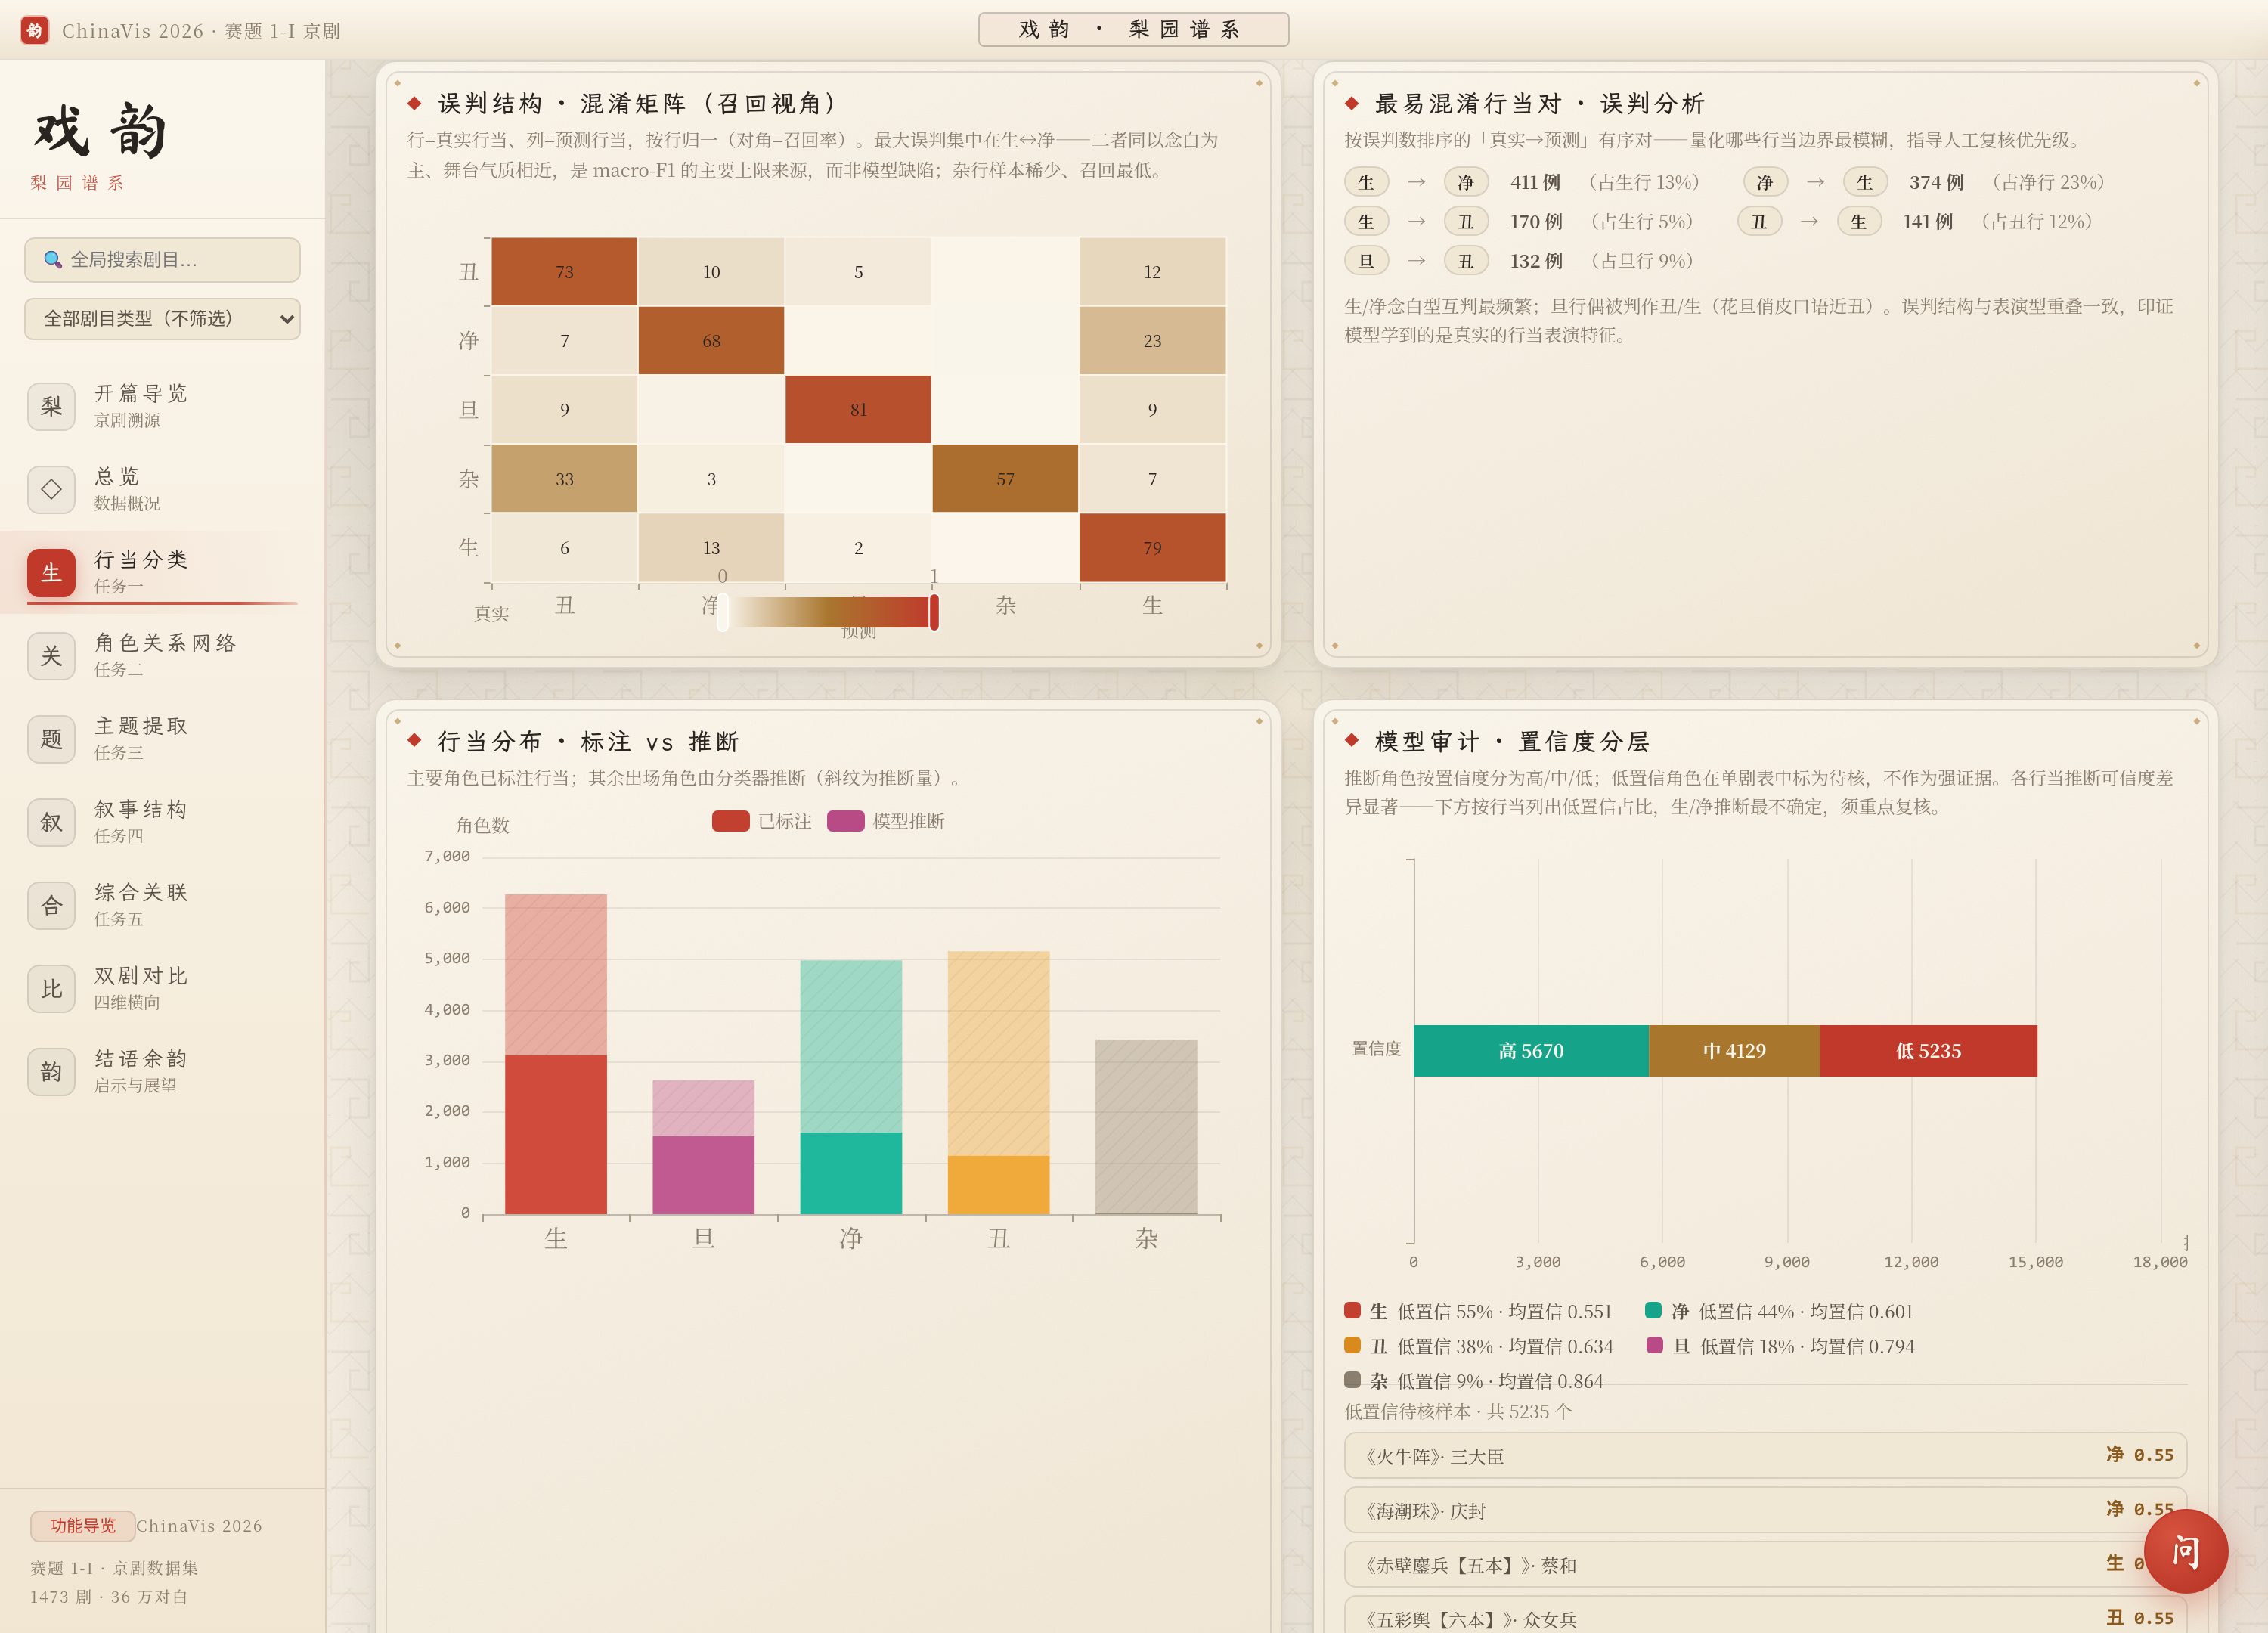
\includegraphics[width=\textwidth]{fig1_roles}
\caption{任务一界面：误判结构混淆矩阵（召回视角）与最易混淆行当对、行当分布、推断置信分层、基线对照与校准曲线。}\end{figure}

\clearpage
\section{角色关系网络结构特征}
\textbf{方法：}以「同场共现 + 对话邻接」定义角色互动——两角色同场出现则加权，相邻发言再加权，过滤台词<2 的龙套堆叠。对 1462 部剧用 networkx 构建关系网络，计算规模、密度、平均度、中心势（Freeman）、聚类系数、模块度与社群数；并按情节/标题关键词将剧目分为历史戏(580)、公案戏(241)、家庭戏(212)、神怪戏(143)、其他(286)。

\textbf{不同剧目类型的网络结构特征：}
\begin{itemize}
\item \textbf{公案戏}网络规模最大（均 15.4 角色 / 68.6 关系）、\textbf{中心势高（0.30，与历史戏并列最高档）}，呈以清官/判官为核心的星型结构，如《狸猫换太子》以包拯为绝对核心（中心性 0.44）。
\item \textbf{历史戏}规模大且\textbf{模块度最高（0.21）}，网络分裂为敌我/朝野多个社群，反映征战剧本的阵营对立结构。为排除「大网络自然模块度高」的混淆，对每剧生成 20 个同规模 Erdős–Rényi 零模型算 $z$ 值，历史戏模块度 $z$=3.23 为各类型最高，证明其社群结构显著强于随机预期。
\item \textbf{家庭戏}规模最小但\textbf{密度最高（0.70）}，人物少而互动紧密。
\item 全库散点显示「网络规模↑则中心势↑」的弱正相关——大戏更依赖核心人物组织剧情。
\end{itemize}

\textbf{结构角色与阵营同质度（按行当聚合）：}逐节点计算度中心性与介数中心性并按行当聚合——\textbf{生行连接最广、介数最高、约 51\% 剧目占据「桥接主座」}（剧情组织者），净次之、杂行最外围。各类型行当同配系数 role assortativity \textbf{均为负（全库 −0.16）}：人物网络按行当「互补异配」（生旦净丑交错搭戏），检测出的社群对应「敌我阵营」而非「同行当抱团」。

\textbf{差异显著性与时期演化：}对各类型指标做两两 Mann–Whitney U 检验（BH-FDR 校正）——历史戏模块度显著高于家庭戏，但与公案、神怪戏差异未达显著（故「模块度并列最高档」更准确）；公案戏规模显著大于其余类型。网络规模随时代\textbf{显著增大}（Kruskal–Wallis 显著，均 10.8→15.4→18.3 角色），人物体系趋于庞大复杂，模块度/中心势在建国初期达峰。

\textbf{结论：}剧目类型在网络拓扑上留下稳定印记——公案重核心、历史重阵营、家庭重密度；行当在结构上分工互补，生行居桥接核心，网络规模随时代增大。

\begin{figure}[h]\centering\includegraphics[width=\textwidth]{fig2_network}
\caption{任务二界面：结构角色散点（度×介数中心性）与各类型行当同配系数、类型差异显著性矩阵（▲显著更高/▼更低/·不显著）、网络结构时期演化曲线。}\end{figure}

\clearpage
\section{核心主题提取与组合模式}
\textbf{方法：}以各剧「情节」摘要（覆盖 99.5\%）为语料，jieba 词性标注仅保留名/动/形内容词。为防主题退化为人名/道具，做两层实体净化：① 用数据自身角色名构建黑名单并补「黄三泰→三泰」等裸名变体；② 按"故事"归并多卷剧（头本/二本/【三本】…）后计文档频率，剔除只在极少数故事出现的剧目专属名/道具（三泰/国母/莲灯/仙果等不再污染主题）。对 K=5…15 扫描 u\_mass 一致性，在 \textbf{K=10} 取得最优后回落，按「一致性退化前最细划分」取 \textbf{K=10}（数据驱动，非硬选粒度）。

\textbf{主题构成与组合：}净化后 10 个主题对应清晰的动作母题——\textbf{征战}（攻打/出战/部将、进京/镇守）、\textbf{忠义复仇}（自刎/报仇/匈奴）、\textbf{婚姻家庭}（夫妻/相府/思念、妻子/投江）、\textbf{断狱}（杀死/状元、乳母/洞房）等。主题共现显示\textbf{征战×忠义复仇}、\textbf{婚姻×家庭}为高频稳定组合。KMeans 得 6 个原型组合，最大原型（约 500 部）以「征战+复仇」动作母题为主干。

\textbf{跨剧本比较：}共性是「家庭/婚姻」母题几乎贯穿各类剧目；差异在于历史戏显著偏向征战/忠义，家庭戏偏向婚姻伦理，公案戏偏向断狱计谋。\textbf{主题随时代迁移}（每剧主题权重 Kruskal–Wallis 检验 + BH-FDR，10 母题占比变化全部显著）：征战类母题随时代\textbf{下降}（攻打/出战 −6.3pt、进京/镇守 −4.2pt），家庭伦理类母题\textbf{上升}（妻子/投江 +7.3pt、母女/父子 +7.6pt）——题材呈现由「武戏征战」向「家庭伦理」的迁移。

\textbf{主题稳健性对照：}以主题-词分布最优匹配余弦衡量复现度——LDA 主题与完全不同的 NMF 方法平均一致 0.46、多 seed LDA 平均一致 0.54，复仇/家庭杀戮/救援等核心母题高度复现（余弦 0.6–0.9），印证「10 母题」非单次随机产物（部分征战母题细分边界有方法依赖性，诚实声明）。

\textbf{结论：}京剧主题表达由少数稳定母题及其有限组合构成，存在「征战—忠义」「婚姻—家庭」等代表性组合模式，与剧目类型强相关，并随时代由武戏向家庭伦理迁移。

\begin{figure}[h]\centering\includegraphics[width=\textwidth]{fig3_topics}
\caption{任务三界面：主题随时代变迁折线（红升/青降）、主题稳健性 NMF/多 seed 对照条、核心主题占比与主题分布图（JS 距离 + MDS）。}\end{figure}

\clearpage
\section{叙事结构与典型叙事模式}
\textbf{方法：}以表演形式标记合成逐场「戏剧强度」曲线——\textbf{唱腔(文)}=该场唱占比、\textbf{武打(武)}=舞台提示中做打动作标记密度（起霸/开打/趟马/圆场…）、\textbf{冲突}=发言人切换率×同场人数；综合强度=0.4·文+0.4·武+0.2·冲突，各按全剧归一。据峰值识别开端/发展/高潮/结局，并将曲线重采样为 16 点后 KMeans 聚类（965 部≥4 场剧目参与）。簇数由 silhouette 选 K=5，并做权重敏感性（±0.1 文武微调 ARI 仍 0.55–0.60，中等稳健）。

\textbf{关键阶段与节奏：}多数剧本经「开端铺陈→逐步累积→后段高潮→收束」推进。全库高潮位置分布右偏、平均渐强指数 +0.10$\sim$0.15，印证戏曲「层层铺垫、后段收束」的惯例。

\textbf{典型叙事模式（5 类，名称互异）：}①平稳铺陈式（288 部）；②结尾陡升式（202 部，峰位≈1.0）；③后段高潮式·渐强（181 部，峰位≈0.8）；④前段先声夺人式（151 部，峰位≤0.34）；⑤中段经典弧线式（143 部，峰位≈0.5）。各原型可叠加簇内 p25–p75 离散度带。\textbf{跨类型差异：}历史戏做打最多（均 5.0）、节奏外放；家庭戏与公案戏更依赖唱念抒情。类型间两两 Mann–Whitney U 检验（BH-FDR）显示：历史戏做打量显著高于家庭戏与神怪戏，但与公案戏差异未达显著——「历史戏做打最多」成立但需限定比较对象，体现诚实的统计判断。

\textbf{结论：}京剧叙事以渐强式后段高潮为主流，并分化出平稳/双段等多种弧线；文武节奏取向与剧目类型紧密对应。

\begin{figure}[h]\centering\includegraphics[width=\textwidth]{fig4_narrative}
\caption{任务四界面：类型节奏差异显著性矩阵（做打量/高潮位置/唱腔占比，▲显著更高/▼更低/·不显著）、5 种典型叙事弧线原型与高潮位置直方。}\end{figure}

\clearpage
\section{综合关联与协同演化}
\textbf{方法：}打通任务二（关系网络）、三（主题）、四（叙事）与行当构成，构建每剧四维联合特征，计算跨维度相关矩阵、「类型→主题→叙事」协同链路（Sankey），并在联合空间用 KMeans 聚出综合原型；提供单剧四维联动档案。对 96 对相关做 Benjamini–Hochberg FDR 校正，\textbf{37 对}在 $p_{\text{adj}}$<0.05 下显著，头条相关全部显著。

\textbf{关联机制（跨维度相关）：}①\textbf{网络规模↔做打量 $r$=+0.58}——人物众多的大网络多承载武戏；②\textbf{模块度↔做打量 +0.45、模块度↔净占比 +0.35}——分阵营的网络对应征战题材、武打高潮、并由净行主导；③\textbf{模块度↔旦占比 −0.32}——旦行为主的戏网络更紧凑单核。

\textbf{偏相关控混淆（甄别真假协同）：}大戏「既人多分阵营、又做打多、又主题杂」，原始相关可能由共同「剧目体量」驱动。对各相关补「控制网络规模/场次后的偏相关」——37 显著项中 \textbf{26 项控体量后仍稳健}。\textbf{行当协同为真}：模块度↔净占比 +0.35→+0.21、↔旦占比 −0.32→−0.22 仍稳健；而 \textbf{「模块度/密度↔做打」实为体量假象}——控体量后衰减到近 0（+0.45→+0.02、−0.51→−0.06），非模块化结构本身偏好武打。\textbf{轻量预测验证}进一步把「协同」升级为「可由 A 预测 B」：仅用非叙事维度（网络+行当+主题）交叉验证预测叙事弧型，macro-F1=0.226 约为多数类基线（0.092）的 2.5 倍——四维确有可预测耦合，但绝对精度不高、叙事保有自身变异。

\textbf{协同链路与稳定结构：}Sankey 显示稳定链路——\textbf{历史戏→征战主题→结尾渐强高潮}、\textbf{家庭戏→婚姻家庭主题→平稳/前段叙事}。联合聚类得 \textbf{6 类综合原型}，如「大网络+征战+武打渐强+净生主导」与「小网络+婚姻+文戏+旦生主导」。

\textbf{结论：}京剧的人物关系、主题表达与叙事方式并非彼此独立，而是存在典型关联模式与协同演化规律——题材决定人物关系拓扑与行当配置，进而塑造叙事节奏。经偏相关控混淆与预测验证，部分协同（行当↔结构）稳健可预测，部分（做打↔结构）实为剧目体量驱动，结论诚实可信。

\begin{figure}[h]\centering\includegraphics[width=\textwidth]{fig5_synthesis}
\caption{任务五界面：跨维度相关热力图，带 $p$ 值/$R^2$/偏相关（控体量 $r$）的关联发现卡（26/37 项控体量后稳健），轻量预测验证（macro-F1=0.226 vs 基线 0.092）。}\end{figure}

\end{document}
